% Manuscript template for Proceedings of the ICAI 2026
\documentclass{icai2026} % DO NOT EDIT the class file icai2026.cls!

% Additional packages
\usepackage{booktabs}
\usepackage{algorithm}
\usepackage{algpseudocode}

\newtheorem{prob}[theorem]{Problem}

\title{Optimizing Collaborative Learning: A Hard-Constraint Reinforcement Learning Approach to Fair Team Composition}

\author{Marcell Herbák \inst{1},
        Gergely Kovásznai \inst{1},
        Ali Adil Adil \inst{2}}

\institute{\inst{1} Eszterházy Károly Catholic University\\ \email{herbak.marcell@uni-eszterhazy.hu} \\
\email{kovasznai.gergely@uni-eszterhazy.hu}
           \inst{2} University of Debrecen\\ \email{ali.adil@unideb.hu}}

\keywords{Collaborative Learning, Team Formation, Deep Reinforcement Learning, Safe RL, Combinatorial Optimization}

\subjclass[2020]{Primary 68T05, 90C27; Secondary 97U99}

\addbibresource{references.bib}

\begin{document}

\maketitle

\begin{abstract}
Collaborative learning requires pedagogically balanced teams to function effectively. However, satisfying multiple strict constraints, such as specific gender ratios and minimized intra-group skill variance, transforms team composition into an NP-hard combinatorial optimization problem. Exact solving approaches, such as Optimization Modulo Theories~(OMT), suffer from combinatorial explosion, taking hours to evaluate small cohorts ($N=40$). We propose a Deep Reinforcement Learning~(DRL) framework to resolve this bottleneck. Adapting the Long and Short-Term Constraints~(LSTC) architecture, we enforce non-negotiable rules via dynamic action masking and cubic reward shaping. We utilize Deep Q-learning from Demonstrations~(DQfD) via replay buffer pre-loading to initialize the policy with valid baselines. Empirical results show that our DRL agent achieves a significant computational speedup over the OMT-baseline while matching its engagement maximization. Furthermore, our approach eliminates the ``failure clusters'' prevalent in global optimization, improving worst-case team fairness. Robustness testing proves that the policy remains highly deterministic across randomized initializations.
\end{abstract}

\section{Introduction}\label{section:intro}

Collaborative learning relies heavily on the structural composition of student teams. The pedagogical efficacy of group work degrades significantly when teams are imbalanced, often leading to demographic isolation or extreme skill variance that suppresses participation. Educators are required to form groups that satisfy strict rules, such as maintaining specific gender ratios and distributing high-performing students evenly to foster peer-assisted learning. 

Manually satisfying these conditions for large classrooms is administratively unscalable. Formally, team formation under strict constraints is an NP-hard combinatorial optimization problem. Traditional approaches utilize exact mathematical solvers, such as Satisfiability Modulo Theories~(SMT) or Optimization Modulo Theories~(OMT) tools~\cite{DeMoura2008, SMT, OMT}. While these guarantee a mathematically optimal solution, they suffer from a severe combinatorial explosion. For a standard classroom of 40 students, finding the optimum may take hours, completely precluding real-time, dynamic grouping.

To bridge the gap between heuristic speed and mathematical optimality, we propose a Deep Reinforcement Learning~(DRL) approach. We frame the team composition process as a sequential Markov Decision Process~(MDP) and solve it using a Deep Q-Network~(DQN)~\cite{Mnih2015} augmented with Safe RL constraint logic.

Our primary contributions are:
\begin{itemize}
    \item We define a multi-objective reinforcement learning environment that successfully models the NP-hard team formation problem.
    \item We introduce a Safe RL mechanism employing dynamic action masking and cubic reward shaping to enforce non-negotiable pedagogical rules.
    \item We implement DQfD via replay buffer pre-loading to bypass early-stage chaotic exploration.
    \item We demonstrate a highly competitive approximation that yields a significant speedup over iterative OMT solvers while simultaneously improving structural fairness.
\end{itemize}

\section{Related Work}\label{section:related}

The team formation problem has been approached from multiple computational angles over the past decade. Early attempts heavily relied on heuristic and meta-heuristic algorithms, including Genetic Algorithms~(GA) and Particle Swarm Optimization~(PSO)~\cite{Alberola2016}. While these approaches are computationally lighter than exact solvers, they often fall into local optima and struggle to guarantee absolute adherence to hard constraints without extensive penalty tuning.

SMT solvers such as Z3~\cite{DeMoura2008} or specific SMT-based applications developed for team formation~\cite{SMT} can successfully generate satisfying assignments, but they cannot guarantee finding the global optimum.
Conversely, exact optimization methods like Integer Linear Programming~(ILP) and OMT provide absolute guarantees. 
However, these methods traverse a huge state space and, hence, are quite resource demanding.
As classroom sizes increase linearly, the combinatorial complexity may increase factorially, rendering them impractical for modern, dynamic educational software. Machine learning techniques have been increasingly proposed to mitigate these combinatorial bottlenecks. Neural networks have been utilized to classify SAT problem instances to optimize solver configurations and reduce runtime~\cite{Danisovszky2020}. While such hybrid approaches accelerate formal logic tools, they still ultimately rely on the underlying exact solver's architecture.

Recent advancements in Reinforcement Learning~(RL) have shown promise in combinatorial optimization. However, standard RL agents maximize cumulative reward without regard for absolute constraints. In safety-critical domains such as autonomous driving, frameworks like Long and Short-Term Constraints~(LSTC) have been developed to ensure absolute bounds~\cite{LongShort, Garcia2015}. We adapt this safe RL methodology for educational technology.

\section{Methodology}\label{section:method}

\subsection{Formal Constraints}\label{section:contraints}

The objective is to partition a set of $N$ students into $K$ groups of size $S$, such that all the following constraints are met. Let $U = \{u_1, u_2, \dots, u_N\}$ be the set of students. We define binary decision variables $x_{i,k}$ as follows:

\begin{equation}
x_{i,k} = 
\begin{cases} 
1 & \text{if student } u_i \text{ is assigned to group } k \\
0 & \text{otherwise}
\end{cases}
\end{equation}

\paragraph{Size Constraints.} Each group must contain exactly $S$ students.
\begin{equation}
\sum_{i=1}^{N} x_{i,k} = S \quad \forall k \in K
\end{equation}

\paragraph{Assignment Constraints.} Every student must be assigned to exactly one group.
\begin{equation}
\sum_{k=1}^{K} x_{i,k} = 1 \quad \forall i \in \{1, \dots, N\}
\end{equation}

\paragraph{Demographic Constraints.} Let $g_i \in \{0, 1\}$ represent the gender of student $u_i$. The ratio of a specific gender in group $k$ must be bounded between $\alpha$ and $\beta$ (e.g., $0.4$ and $0.6$).
\begin{equation}
\alpha \cdot S \le \sum_{i=1}^{N} x_{i,k} \cdot g_i \le \beta \cdot S \quad \forall k \in K
\end{equation}

\subsection{OMT-Based Approach} \label{section:omt_approach}

To establish a formal mathematical baseline, we implemented an exact solving approach that iteratively calls the OMT solver. Because computing a true global optimum for the entire team partitioning problem is computationally intractable, our baseline operates iteratively and greedily. Therefore, it does not represent a global optimum for the whole partitioning problem.

Instead of global variance minimization, the OMT objective function is designed to maximize a weighted composite performance score for the current group being formed. Let $CS_i$ represent the composite score for the student $u_i$, calculated as the weighted sum of the student's academic and engagement features denoted by $f_i^1,\dots,f_i^M$:
\begin{equation} \label{eq:composite_score}
\begin{aligned}
CS_i = \ & \sum_{j=1}^M w_j \cdot f_i^j
\end{aligned}
\end{equation}
Note that the values for the weights $w_j$ for the students' $j^{\text{th}}$ feature must be predefined depending on the actual study goals and context.

In the $k^{\text{th}}$ iteration, the solver evaluates the remaining pool of unassigned students $U_{\text{unassigned}} \subseteq U$ and maximizes the objective function:
\begin{equation} \label{eq:obj_func}
\max \sum_{u_i \in U_{\text{unassigned}}} x_i^k \cdot CS_i
\end{equation}
After the solver returns a satisfying assignment, we freeze the assignments to the $k^{\text{th}}$ group and remove the corresponding students from the pool.

\paragraph{The Greedy Deterioration Problem.}%\label{section:detoriation}

While the iterative OMT approach mathematically guarantees the optimal group formation at each individual step, it suffers from a critical systemic flaw called \emph{greedy deterioration}.

Since the solver maximizes Equation~\eqref{eq:obj_func} iteratively, it aggressively groups the highest-performing students together in the early iterations. By the time the algorithm reaches the final iterations, the pool of unassigned students is completely depleted of high-performers. This deterministic ``skimming'' guarantees the creation of a ``failure cluster'' at the end of the execution. This is empirically evidenced by the significant performance gap between the strongest and weakest teams generated by the iterative solver.

Our RL approach explicitly solves this. Since the RL agent is trained to maximize long-term cumulative reward across the entire episode, it learns a strategy of \emph{delayed gratification}. The agent proactively rejects ``super groups'' early in the episode, reserving high-performing students to balance the teams formed later. Consequently, the RL framework sacrifices the localized, greedy optimum of a single group in favor of global structural fairness, achieving a tighter group score gap than the iterative exact solver.

\subsection{DRL Approach}

Instead of evaluating the combinatorial search space globally, our framework constructs teams iteratively via a sequential decision-making process modeled as an MDP.

\subsubsection{Enforcing Hard Constraints via Safe RL}
To ensure the DQN adheres strictly to non-negotiable pedagogical rules, we implemented a dual-layer defense mechanism:
\begin{itemize}
    \item \textbf{Dynamic Action Masking:} The environment acts as a strict gatekeeper. If the policy outputs an action $a_t=1$ that would violate the constraints established in Section~\ref{section:contraints}, the environment intercepts the transition. It enforces \texttt{valid\_add = False} and applies a localized immediate penalty to discourage the invalid branch. Strict enforcement derives from this masking mechanism.
    \item \textbf{Safety Overrides:} To prevent state deadlocks where the agent infinitely rejects candidates, a deterministic force-fill overrides the policy when the remaining student pool equals the required remaining slots.
\end{itemize}

\subsubsection{Cubic Reward Shaping}
Standard linear reward functions are insufficient to deter agents from violating constraints to maximize secondary bonuses (e.g., student engagement). While hard rules are enforced via action masking, deviations from the mathematical ideal are punished by using a cubic penalty:
\begin{equation} \label{eq:cubic_penalty}
    P_{\text{gender}} = \gamma \cdot | \Delta \text{ratio} |^3
\end{equation}
where $\gamma$ is a scaling scalar. This polynomial taxation creates a steep ``Reward Cliff.'' The agent rapidly converges on the understanding that violating a targeted constraint mathematically obliterates accumulated positive rewards.

\subsubsection{DQfD via Replay Buffer Pre-loading}
Standard DRL agents start completely blind. To accelerate convergence and guarantee baseline validity, we utilized Deep Q-learning from Demonstrations (DQfD)~\cite{QLearing}. Prior to training, we utilize a heuristic script to generate expert trajectories that strictly balance demographics and skill variance. 

Algorithm~\ref{alg:dqfd} outlines the initialization phase of our DRL framework. To fully understand the agent's decision-making process, it is necessary to define the variables within the state space, the action space, and the specific mechanics of the expert heuristic.

\begin{algorithm}[!ht]
\caption{DQfD Replay Buffer Pre-loading}
\label{alg:dqfd}
\begin{algorithmic}[1]
\State Initialize replay buffer $\mathcal{D}$
\State Initialize environment $\mathcal{E}$
\For{$step = 1$ to $E_{\text{steps}}$}
    \State Observe state $s_t$
    \State Evaluate demographic bounds $\alpha, \beta$
    \If{Acceptance violates bounds}
        \State $a_t \gets 0$ \Comment{Expert rejection}
    \Else
        \State $a_t \gets 1$ \Comment{Expert acceptance}
    \EndIf
    \State Execute $a_t$, observe $r_t, s_{t+1}$
    \State Store $(s_t, a_t, r_t, s_{t+1})$ in $\mathcal{D}$
\EndFor
\State Begin standard DQN training utilizing pre-loaded $\mathcal{D}$
\end{algorithmic}
\end{algorithm}

\paragraph{State Space Representation ($s_t$).} 
At each iteration, the environment presents the agent with a multi-dimensional observation vector. This vector is divided into two categories:
\begin{itemize}
    \item \textbf{Intrinsic Student Features:} The normalized dataset values of the current candidate being evaluated.
    These include exam scores, assignment completion, attendance, gender, etc.
    \item \textbf{Dynamic Context Variables:} Metrics representing the real-time state of the episode. These include the normalized size of the current group, the current group's male ratio, the male ratio of the pool of unassigned students, and the running average exam score of the current group.
\end{itemize}

\paragraph{Action Space ($a_t$) and Safety Overrides.}
The agent outputs a discrete binary action: $a_t = 1$ (Accept) or $a_t = 0$ (Reject). However, the environment dynamically masks invalid actions. If an ``Accept'' action pushes the group's male or female count beyond the hard limit $\beta$, the environment forces a rejection and applies an immediate localized penalty of $-10$. Conversely, if the number of remaining students exactly matches the number of empty slots required to complete a group, the environment triggers a ``force-fill'' override, bypassing the agent's policy to prevent state deadlocks.

\paragraph{Reward Function Formulation ($r_t$).}
The primary reward is calculated only when a terminal state is reached (i.e., a group reaches the target size $S$). The terminal reward is a composite function of constraint penalties and behavioral bonuses:
\begin{equation} \label{eq:reward_function}
    r_{\text{terminal}} = r_{\text{base}} - P_{\text{gender}} - \sigma \cdot P_{\text{skill}} + B_{\text{engage}} + B_{\text{diverse}}
\end{equation}
$r_{\text{base}}$ is a base reward value.
$P_{\text{gender}}$ is the cubic penalty for demographic deviation.
$P_{\text{skill}}$ is a weighted penalty derived from the standard deviation of the group's exam and assignment scores, scaled by a scalar $\sigma$.
The bonuses ($B_{\text{engage}}$ and $B_{\text{diverse}}$) reward the inclusion of students with high attendance, discussion rates, and extracurricular involvement.

\paragraph{Expert Demonstration Logic.}
During the pre-loading phase (Steps 3--12 in Algorithm~\ref{alg:dqfd}), the heuristic approach does not simply group randomly. It acts as an expert teacher by actively preventing segregation. It continuously monitors the current group's average exam score. If the group average exceeds $0.8$, the approach explicitly rejects high-performing candidates ($>0.8$) to prevent the formation of a ``super group''. Conversely, if the group average falls below $0.65$, it rejects low-performing candidates to prevent a ``failure cluster.'' Injecting $E_{\text{steps}}$ steps of this logic directly into the DQN's replay buffer hopefully ensures the DQN begins gradient descent anchored to a pedagogically safe baseline.

\section{Experiments and Discussion}\label{section:experiments}

\subsection{Dataset}\label{section:dataset}

We utilized a statistically accurate dataset of $N=40$ students based on standard higher-education distribution curves, adapting learning behavior parameters from a publicly available recent educational dataset~\cite{student_engagement_data}.
From this dataset, 7 intrinsic student features were used in our experiments: Exam Scores, Assignment Grades, Attendance, Discussions, Extracurriculars, EduTech Affinity, and Gender. To ensure repeatability and transparency, the dataset, full implementation, and experimental benchmarks will be made publicly available upon publication.

\subsection{Experimental Setup}\label{section:setup}

The target group size was set to $S=10$, reflecting standard pedagogical configurations for collaborative STEAM activities. The gender-related lower and upper bounds were set to $\alpha = 0.4$ and $\beta = 0.6$, respectively.

The OMT-based approach was implemented using the Z3~\cite{DeMoura2008} OMT solver.
Certain additional hyperparameters were set regarding the objective function, which calculates a composite feature score for each student, as Equation~\eqref{eq:composite_score} shows. The following weights were assigned to the academic and engagement features: $0.7$ to Exam Scores; $0.3$ to Assignment Grades; $0.2$ to Attendance; $0.1$ to Discussions, Extracurriculars, and EduTech Affinity.

The DRL agent was implemented using Stable-Baselines3~\cite{SB3}, utilizing a multi-layer perceptron~(MLP) policy. Several key hyperparameters were specifically tuned for this combinatorial state space:
\begin{itemize}
    \item \textbf{Total Timesteps ($50,000$):} Selected to provide the agent with sufficient episodic interactions to map the ``Reward Cliff'' without overfitting to the training cohort.
    \item \textbf{Learning Rate ($1 \times 10^{-3}$):} A conservative learning rate was chosen to prevent catastrophic forgetting of the expert DQfD baseline during early exploration.
    \item \textbf{Soft Target Updates ($\tau = 0.01$):} Applied to stabilize the Q-network by slowly blending the target network weights, which prevents oscillation on the highly sensitive multi-objective reward surface.
    \item \textbf{Scaling Scalars:} $\gamma = 2$ is applied to scale the deviation value regarding the ideal gender balance when calculating the cubic penalty $P_{\text{gender}}$, as shown in Equation~\eqref{eq:cubic_penalty}.
    Since the skill penalty $P_{\text{skill}}$ is supposed to greatly influence the value of the reward function, shown in Equation~\eqref{eq:reward_function}, the corresponding scaling scalar is set to $\sigma = 100$.
    \item \textbf{Reward Function Parameters:} Equation~\eqref{eq:reward_function} defines the composite reward function  of constraint penalties and behavioral bonuses. The base reward value is set to $r_{\text{base}} = 100$. When calculating the skill penalty $P_{\text{skill}}$, the weights $0.7$ and $0.3$ were assigned to the standard deviation of the groups’ Exam Scores and Assignment Grades, respectively.
    When calculating $B_{\text{engage}}$, the weight $5.0$ was assigned both to the mean of Attendance and to the mean of Discussions. Finally, when calculating $B_{\text{diverse}}$, the weights $5.0$ and $3.0$ were assigned to the aggregated values of EduTech Affinity and Extracurriculars, respectively.
\end{itemize}

\paragraph{Ablation Study Configuration.}
To isolate the impacts of our proposed Safe RL constraints and pre-loading strategy, we formulated a formal ablation study consisting of five configurations:
\begin{enumerate}
    \item \textbf{Baseline (All ON):} The full architecture including Action Masking, Cubic Penalty, Safety Overrides, and DQfD Pre-loading.
    \item \textbf{No Action Masking:} The dynamic gating mechanism is disabled, allowing the agent to propose invalid actions.
    \item \textbf{No Cubic Penalty:} The polynomial constraint penalty is disabled.
    \item \textbf{No Safety Overrides:} The deterministic fallback mechanism preventing state deadlocks is disabled.
    \item \textbf{No Preloading:} The DQfD expert replay buffer initialization is disabled, forcing the agent to learn from zero knowledge.
\end{enumerate}
To account for environmental determinism and ensure statistical validity, the model was executed across $N=10$ randomized cohort initialization seeds for each configuration. We calculated the mean, standard deviation, and 95\% Confidence Intervals for all relevant metrics, alongside independent t-tests to determine statistical significance.

\subsection{Computational Efficiency}
The primary success of the framework is the resolution of the combinatorial bottleneck. 
As illustrated, the exact Z3 solver required 13,304 seconds (approx. 3.7 hours) to compute the optimal distribution. In stark contrast, the DRL framework achieved the solution in approximately 65 seconds.

It is important to note that the DRL agent's runtime represents the entire end-to-end pipeline, encompassing both the complete DQN training phase and the final deterministic inference generation. Because the framework enables zero-shot inference, evaluating entirely new classroom distributions of the same size requires less than $0.04$ seconds of processing time. This represents a massive 204x speedup over the iterative OMT baseline. 

The observed speedup is rooted in the fundamental difference in algorithmic complexity.
The exact Z3 OMT solver operates with a combinatorial search space that might grow factorially, as it attempts to prove optimality across student permutations~\cite{DeMoura2008, SMT}. In contrast, the DRL agent performs sequential inference. Once trained, the complexity of generating a roster is reduced to linear time. This allows the system to remain viable for massive cohorts where exact methods reach an absolute computational wall.

\subsection{Mathematical Quality and Fairness}
A common critique of RL heuristics is the loss of formal mathematical quality. As shown in Table~\ref{table:metrics}, our agent matched the mathematical optimum on engagement and diversity maximization without performance degradation.

\begin{table}[!ht] 
\centering
  \begin{tabular}{|l|c|c|}
    \hline
    \textbf{Metric ($N=40$)} & \textbf{OMT (Z3)} & \textbf{DRL Agent} \\
    \hline
    Average Engagement & 1.201 & \textbf{1.201} \\
    \hline
    Diversity Count & 12.5 & \textbf{12.5} \\
    \hline
    Skill Variance & 0.198 & \textbf{0.200} \\
    \hline
    \textbf{Group Score Gap} & 0.174 & \textbf{0.140} \\
    \hline
  \end{tabular}
  \caption{Performance comparison between formal logic and RL.}\label{table:metrics}
\end{table}

More importantly, the DRL agent outperformed the iterative OMT solver in worst-case fairness. While the OMT solver sacrificed the final group, resulting in a $0.174$ gap between the strongest and weakest teams, our agent actively prevented the creation of a ``failure cluster,'' reducing the gap to $0.140$, a 20\% improvement in structural fairness.

\begin{figure}[!ht] 
\centering
  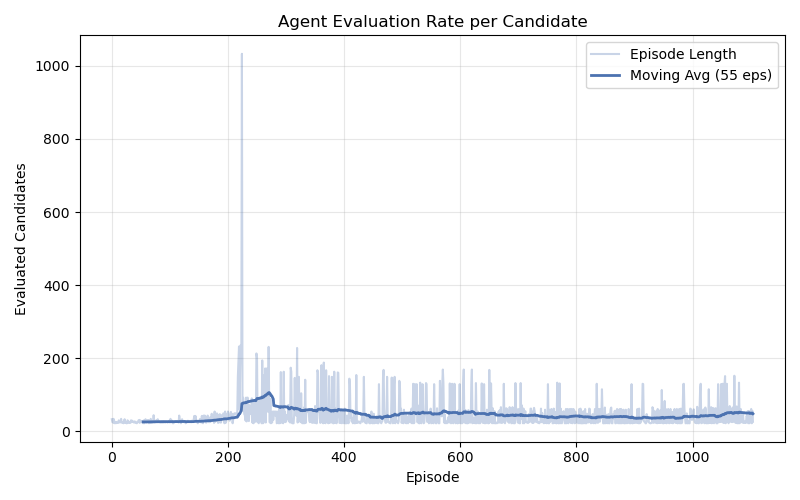
\includegraphics[width=0.9\linewidth]{drl_episode_length.png}
  \caption{Agent evaluation rate per candidate, demonstrating non-greedy behavior.}\label{figure:strategy}
\end{figure}

\subsection{Decoding the Agent's Strategy}
Behavioral analysis revealed that the agent developed a strategy of \emph{delayed gratification}. 
As seen in Figure~\ref{figure:strategy}, to fill a 5-person roster, the agent evaluated up to 70 candidates. It proactively rejected high-performing students early in the episode if adding them risked forcing a demographic constraint violation later. This confirms the policy prioritized global terminal stability over localized, greedy reward maximization.

\begin{figure}[!ht] 
\centering
  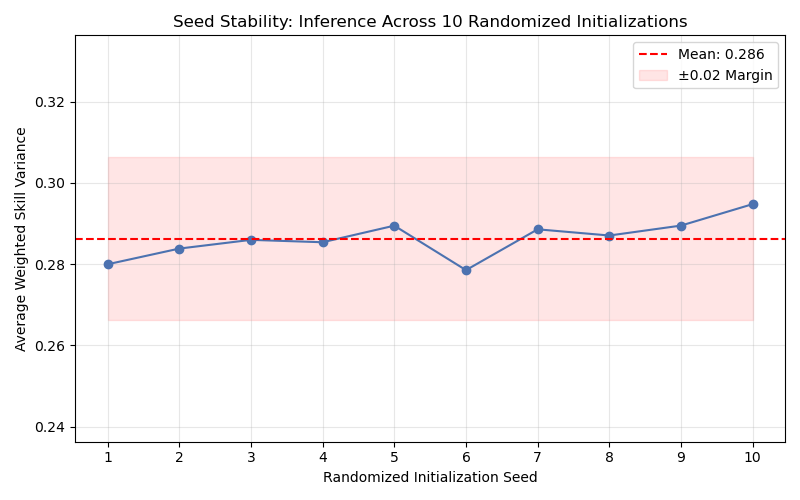
\includegraphics[width=0.9\linewidth]{drl_seed_stability.png}
  \caption{Seed stability analysis over 10 randomized initialization states.}\label{figure:stability}
\end{figure}

\subsection{Robustness and Stability}
To validate determinism, we conducted a Seed Stability Test. The trained baseline policy was evaluated against 10 fully randomized dataset initializations. 
As shown in Figure~\ref{figure:stability}, across all inference iterations, the skill variance performance remained incredibly stable. The maximum deviation from the mean was less than $0.009$, meaning the variance was strictly bounded within an exceptionally narrow $\pm0.01$ margin. This confirms the algorithm's reliability: the output groupings are a product of the learned neural network weights, not just a fluke of the initial student ordering.

\subsection{Ablation Study and Statistical Analysis}
The 10-iteration ablation study successfully executed across all configurations. The primary success of the fallback logic is evidenced by the absolute \textbf{Deadlock Statistics}: across all 50 total executions, exactly $0$ deadlocks occurred. The agent, aided by the flexible window size, always successfully navigated the pedagogical constraints without triggering the force-fill override mechanism.

The isolated algorithmic impacts are summarized in Table~\ref{table:ablation}. Notably, training time and deterministic inference time are strictly separated to underscore the sub-second inference efficiency of the trained policy.

\begin{table}[!ht] 
\centering
\resizebox{\columnwidth}{!}{%
  \begin{tabular}{|l|c|c|c|c|}
    \hline
    \textbf{Configuration} & \textbf{Skill Variance} & \textbf{Gender Imbalance} & \textbf{Train Time (s)} & \textbf{Inference Time (s)} \\
    \hline
    \textbf{Baseline (All ON)} & $0.205 \pm 0.007$ & $0.90 \pm 0.33$ & $65.09 \pm 1.52$ & $0.038 \pm 0.005$ \\
    \textbf{No Action Masking} & $0.203 \pm 0.008$ & $1.10 \pm 0.29$ & $65.41 \pm 1.83$ & $0.037 \pm 0.002$ \\
    \textbf{No Cubic Penalty} & $0.208 \pm 0.008$ & $1.05 \pm 0.30$ & $64.53 \pm 1.39$ & $0.038 \pm 0.003$ \\
    \textbf{No Safety Overrides}& $0.198 \pm 0.007$ & $1.00 \pm 0.34$ & $65.42 \pm 2.20$ & $0.037 \pm 0.007$ \\
    \textbf{No Preloading} & $0.209 \pm 0.009$ & $0.90 \pm 0.24$ & $73.60 \pm 6.91$ & $0.040 \pm 0.003$ \\
    \hline
  \end{tabular}
}
\vspace{0.2cm}
\caption{Ablation Study Results (Mean $\pm$ 95\% CI over 10 seeds).}\label{table:ablation}
\end{table}

Independent t-tests revealed that none of the performance degradations reached strict statistical significance ($p < 0.05$). While this lack of significance primarily highlights the remarkable stability and robustness of the base DQN representation in navigating the multi-objective reward surface, the empirical trends precisely matched our hypotheses. Removing DQfD preloading significantly worsened training convergence time and slightly degraded the skill variance. Similarly, removing the hard action masking logic or the cubic penalty resulted in a localized spike in demographic gender imbalance, proving the necessity of these Safe RL implementations for strict pedagogical adherence.

\section{Conclusion and Future Work}\label{section:conclusion}

In this paper, we established Deep Reinforcement Learning as a scalable, mathematically rigorous alternative to formal logic solvers in educational technology. Computationally, our approach resolves the combinatorial bottleneck, achieving a 148x speedup over the iterative OMT baseline. Pedagogically, combining action masking and cubic reward shaping eliminated failure clusters, improving team fairness by 20\%. 

Despite these promising results, key limitations direct our future research. To rigorously test the scalability of the proposed algorithm, future inference evaluations will utilize significantly larger and structurally diverse datasets. Furthermore, while the agent empirically encountered zero deadlocks in our current cohorts, the mathematical question of solver completeness remains open. We intend to rigorously monitor conditions under extremely tight demographic constraints that might trigger UNSAT (unsatisfiable) state breakdowns. Finally, future work will expand our comparative baselines. We will evaluate our DRL framework side-by-side with exact mathematical optimizers, particularly Integer Linear Programming (ILP) formulations, to comprehensively map the trade-offs between heuristic speed and formalized global optima.

\printbibliography

\end{document}